\chapter{Hybrid Context-Sensitivity}
\label{chapter:hybrid}
\epigraph{If you wanted to know about the Hybrid, why didn’t you just ask me?}{\textit{The 12th Doctor} - Doctor Who}

Although in principle call-site- and object-sensitivity are incomparable, in practice the story is quite clear. Call-site-sensitivity has a long history, dating to at least the '80s. For a long time, call-site-sensitivity was considered synonymous with context-sensitivity as a whole. Object-sensitivity was later introduced in 2002 \cite{issta:2002:Milanova} and within a decade it has become the overwhelming choice of context-sensitivity for object-oriented programs. Multiple studies \cite{pldi:2006:Naik,paste:2005:Liang,thesis:Lhotak,article:2008:tosem:Lhotak,oopsla:2009:Bravenboer} have found object-sensitive analyses to yield excellent precision/cost tradeoffs. Compared to call-site-sensitive analyses, an object-sensitive analysis of the same context depth has always been advantageous, in terms of both speed and performance.

Given such past experimental results, it would seem that exploring combinations of call-site- and object-sensitivity is futile. There is no tradeoff to exploit. Even though call-site-sensitive analyses are occasionally faster to execute, this only comes at the expense of precision. To achieve the same precision level as an object-sensitive analysis, call-site-sensitive analyses have to suffer much higher cost. Additionally, coarser approximations of object-sensitivity, such as \emph{type-sensitivity} \cite{popl:2011:Smaragdakis} have filled the performance gap and offered fast options for cases when a full object-sensitive analysis is too expensive.

The question behind this chapter is whether the two kinds of context can be fruitfully combined, given how dissimilar they are. In order to address this question, we map the design space of \emph{hybrid} call-site- and object-sensitive analyses and describe the combinations that arise. Our work shows that the aforementioned conventional wisdom is false. This is one of the rare occasions when the combination of two ideas supplants both: hybrid context-sensitivity outperforms both object- and call-site-sensitivity in both precision and speed.

Naive hybrid combinations, such as always maintaining as context \emph{both} call and allocation sites, do not pay off, due to extremely high cost. For instance, keeping one call-site and one allocation site as context, in all places, yields a very expensive analysis, on average 3.9x slower than a simple 1-object-sensitive analysis. Although such a combination will improve precision, it is still lacking in comparison to, for example, a 2-object-sensitive analysis.

However, we find that more sophisticated hybrids are highly beneficial. Specifically, we show that we can switch per-language-feature between a combined context and an object-only context. For instance, contexts for static method calls are computed differently from contexts for dynamic method calls. This approach yields analyses with both low cost and high precision. Furthermore, adapting contexts per program feature defines a complex design space and allows even further optimization. Design choices arise, such as, how should the context adapt when a dynamic method call, or an object allocation are made inside a static method?

The end result is analyses that closely track the precision of a combined call-site-and-object-sensitivity while incurring none of the cost. In fact, the cost of the resulting analysis is usually \emph{less} (and occasionally much less) than that of just an object-sensitive analysis, due to increased precision. This effect is shown to apply widely, to several variants of analyses. Accordingly, this outcome establishes new sweet spots for the analyses most relevant for practical applications: 1-object-sensitive, 2-object-sensitive with a 1-context-sensitive heap, and analogous type-sensitive \cite{popl:2011:Smaragdakis} analyses. For all of them, a selective hybrid context is typically both more precise and faster than the original analysis.

In all, this chapter describes the following contributions:

\begin{itemize}
\item \todo{} We model the parameter space of context-sensitive points-to analysis in a way that allows both call-site- and object-sensitivity, as well as combinations and switching of context at key points (in our case study, virtual calls vs. static calls). In this space, we map out choices that produce entirely different flavors of algorithms.

\item We introduce the idea of hybrid call-site- and object-sensitivity where the two kinds of context are freely mixed and the mix is adjusted in response to analyzing different program features. The goal is to achieve the precision of keeping \emph{both} kinds of context together, but at the same cost as keeping only one.

\item We implement our approach in the \doop{} framework and apply it to a large variety of algorithms with varying context depth.

\item We show experimentally, over large Java benchmarks and the Java JDK, that hybrid context-sensitivity works remarkably well. Our experiments establish that different programming language constructs are best analyzed with different kinds of context. The selective application of a combined context achieves the same \emph{effective} precision as keeping both contexts at all times, at a fraction of the cost, and is typically faster even than keeping only an object context. For instance, in the practically important case of a 2-object-sensitive analysis with a context-sensitive heap, we get an average speedup of 1.53x \emph{and} a more precise analysis. Similarly, for the simple and popular 1-object-sensitive analysis, we get an average speedup of 1.12x combined with significant increase in precision.
\end{itemize}


\section{Hybrid Context-Sensitive Analyses}
\label{sec:hybrid:main}

We can now explore interesting combinations of call-site- and object-sensitivity. The design space is large and we will be selective in our presentation and later experiments. Our choice of analyses in this space leverages insights from past studies on what kinds of context are beneficial.\footnote{We have validated these insights with extensive measurements on our experimental setup, and have generally explored a much larger portion of the design space than is possible to present in our evaluation section.} Such insights include:

\begin{itemize}
\item A call-site-sensitive heap is far less attractive than an object-sensitive heap. Generally, adding a heap context to a call-site-sensitive analysis increases precision very slightly, compared to the overwhelming cost.

\item When there is a choice between keeping an object-context or a call-site-context, the former is typically more profitable. This is well validated in extensive past measurements by Lhot\'{a}k and Hendren~\cite{article:2008:tosem:Lhotak}, comparing call-site-sensitive and object-sensitive analyses of various depths. In other words, call-site-sensitivity is best added as \emph{extra} context over an object-sensitive analysis and will almost never pay off as a replacement context, for an object-oriented language.
\end{itemize}


\subsection{Uniform Hybrid Analyses}

The first kind of context combination is a straightforward one: both kinds of context are kept. We term such combinations \emph{uniform hybrid analyses}. In the variants we describe, a uniform hybrid analysis is guaranteed to be more precise\footnote{We use the term ``more precise'' colloquially. Strictly speaking, the analysis is guaranteed to be ``at least as precise'' and not necessarily ``more''.} than the base analysis being enhanced. The question is whether such precision will justify the added cost.

The insight is that by using every information available at each point we can get more precise analyses. Although that is proved to be true, experimental results also show that this precision gain comes with an infeasibly high cost in most cases. Still, we present some analyses that fully combine call-site and object sensitivity as a middle step for understanding later improvements and also as a baseline when comparing more elaborate ways of context combination.

\paragraph[Uniform 1-object-sensitive]{Uniform 1-object-sensitive hybrid (U-1obj).}
Enhancing a 1-object-sensitive analysis with call-site sensitivity results in an analysis with an empty heap context (\args{HC} = \args{\{$\star$\}}) but with a context that consists of both the allocation site of the receiver object and the invocation site of the method (\args{C} = \args{H $\times$ I}). The following definitions describe the analysis:

\begin{quote}
\cons{Record}{heap, ctx}{$\star$} \\
\cons{Merge}{heap, hctx, invo, ctx}{\bl{pair}(heap, invo)} \\
\cons{MergeStatic}{invo, ctx}{\bl{pair}(\bl{first}(ctx), invo)} 
\end{quote}

In words: a virtual method has as context the abstraction of its receiver object, extended with the method's invocation site.  A static method keeps a context consisting of the most significant part of the caller's context and the method's invocation site. Note that under the above definitions, the context of a U-1obj analysis is always a superset of that of 1obj, hence the analysis is strictly more precise.

\paragraph[Uniform 2-object-sensitive with 1-context-sensitive heap]{Uniform 2-object-sensitive with 1-context-sensitive heap hybrid (U-2obj+H).}
A 2-object-sensitive analysis with a context-sensitive heap can be enhanced in the same way. A heap context consists of an allocation site (\args{HC} = \args{H}) and a method context consists of two allocation sites and one invocation site (\args{C} = \args{H $\times$ H $\times$ I}).  The constructor definitions for the analysis are:

\begin{quote}
\cons{Record}{heap, ctx}{\bl{first}(ctx)} \\
\cons{Merge}{heap, hctx, invo, ctx}{\bl{triple}(heap, hctx, invo)} \\
\cons{MergeStatic}{invo, ctx}{\bl{triple}(\bl{first}(ctx), \bl{second}(ctx), invo)} 
\end{quote}

In words: an object's heap context is the receiver object of the method doing the allocation. A virtual method's context is its receiver object's allocation site and context (the latter being the allocation site of the object that allocated the receiver), followed by the invocation site of the method. On a static call, the heap part (i.e., first two elements) of the method context is kept unchanged, and extended with the invocation site of the call.

This analysis is also strictly more precise than the ``plain'' analysis it is based on, 2obj+H. This is achieved partly by placing the receiver object's allocation site in the most significant position of the context triple. In this way, the \consname{Record} function produces the same heap context as 2obj+H on an object's allocation. Alternative definitions are possible for the same sets of contexts, \args{C} and \args{HC}. For instance, one could choose to place \args{hctx} in the most significant position. Similarly, one could produce a hybrid analysis based on 2obj+H but with a different kind of heap context, e.g., \args{HC} = \args{I}, therefore using the invocation site in a method's context as an allocation context. These definitions make decisively less sense, however, per the insights mentioned earlier: invocation sites are rarely advantageous as heap contexts, and, similarly, it is not reasonable to invert the natural significance order of \args{heap} vs. \args{hctx}. (We have also verified experimentally that such combinations yield bad analyses.)

Note here that in deeper analyses where some elements from the context are used in order to create new heap contexts, it is important which ones we choose to propagate. Different choices might result in analyses that behave quite differently both in terms of performance and precision. We can easily influence which context elements are selected for propagation, by changing their ordering in the context.

\paragraph[Uniform 2-type-sensitive with 1-context-sensitive heap]{Uniform 2-type-sensitive with 1-context-sensitive heap hybrid (U-2type+H).}
Isomorphically to object-sensitivity, we can enhance type-sensitive analyses with call-site information in the same way. When applied to a 2-type-sensitive analysis with a context-sensitive heap, this results in an analysis with a heap context of one type (\args{HC} = \args{T}) and a context of two types and an invocation site (\args{C} = \args{T $\times$ T $\times$ I})---mirroring the 2-object-sensitive analysis with a context sensitive heap. The definitions are almost identical:

\begin{quote}
\cons{Record}{heap, ctx}{\bl{first}(ctx)} \\
\cons{Merge}{heap, hctx, invo, ctx}{\bl{triple}($\mathcal{C_A}$(heap), hctx, invo)} \\
\cons{MergeStatic}{invo, ctx}{\bl{triple}(\bl{first}(ctx), \bl{second}(ctx), invo)} 
\end{quote}


\subsection{Selective Hybrid Analyses}

Another approach to hybrid call-site- and object-sensitive analyses is to maintain a context that varies inside the same analysis. We call such analyses \emph{selective hybrid analyses}, as opposed to the earlier ``uniform hybrid'' ones. In a selective hybrid analysis, the sets of contexts, \args{C} and \args{HC}, will be formed as the cartesian (\todo{}) product of unions of sets. Depending on the information available at different analysis points where new contexts are formed, we shall create contexts of a different kind, instead of always keeping a combination of rigid form. We have already hinted at such opportunities in Section~\ref{sec:intro:model-instances}: at a static method call, an object-sensitive analysis does not have a heap object available to create a new context, hence it can at best propagate the context of the caller. Yet, an invocation site is available and can be used to distinguish different static calls, as long as we are allowed to use it as context. This observation generalizes: static invocations are a language feature that benefits highly from the presence of call-site-sensitive elements in the context. This is not hard to explain: For object-sensitive analyses, when analyzing a static invocation, we do not have much information to use in creating a new context, in contrast to a ``normal'' virtual invocation. Consequently, it is beneficial to be able to use the invocation site as a differentiator of static calls.

Selective hybrid analyses are among the most interesting parts of our work and, to our knowledge, have never before arisen in the literature, far less specified, implemented, and evaluated.

\paragraph[Selective 1-object-sensitive (-A)]{Selective 1-object-sensitive hybrid A (S$_A$-1obj).}
Trying to selectively enhance a 1-object-sensitive analysis (\args{HC} = \args{\{$\star$\}}) with call-site sensitive elements, we are presented with two options, relative to how contexts are created in static invocations. The first option is quite simple: we can keep only a single context element in both virtual and static invocations. Consequently, in virtual invocations the context will be an allocation site, but in static invocations it will be an invocation site (\args{C} = \args{H $\cup$ I}). The definitions needed are the following:

\begin{quote}
\cons{Record}{heap, ctx}{$\star$} \\
\cons{Merge}{heap, hctx, invo, ctx}{heap} \\
\cons{MergeStatic}{invo, ctx}{invo} 
\end{quote}

Note that this analysis is \emph{not} guaranteed to be more precise than the 1obj analysis it is based on. Nevertheless, it should be an excellent reference point for comparison and insights: it will suggest how much precision can be gained or lost by call-site-sensitivity as a replacement of object-sensitivity in static method calls.

\paragraph[Selective 1-object-sensitive (-B)]{Selective 1-object-sensitive hybrid B (S$_B$-1obj).}
The second option for a selective hybrid enhancement of a 1-object-sensitive analysis is to add \emph{extra} information to the context of static calls. This means that context in virtual invocations is still an allocation site, but context in static invocations now consists of both the allocation site copied from the caller \emph{and} the invocation site. In this way, \args{C} = \args{H $\times$ (I $\cup$ \{$\star$\})}. That is, the context can be either just an allocation site or an allocation site and an invocation site. (This could also be written equivalently as \args{C} = \args{H $\cup$ (H $\times$ I)}, but the earlier form streamlines the definitions of constructors, as it makes all contexts be pairs, thus avoiding case-based definitions.)  In this way the constructor definitions become:

\begin{quote}
\cons{Record}{heap, ctx}{$\star$} \\
\cons{Merge}{heap, hctx, invo, ctx}{\bl{pair}(heap, $\star$)} \\
\cons{MergeStatic}{invo, ctx}{\bl{pair}(\bl{first}(ctx), invo)}
\end{quote}

This analysis has a context that is always a superset of the 1obj context and, therefore, is guaranteed to be more precise.

\paragraph[Selective 2-object-sensitive with 1-context-sensitive heap]{Selective 2-object-sensitive with 1-context-sensitive heap hybrid (S-2obj+H).}
When dealing with deeper analyses, the possible design decisions start to vary. For example, for a 2-object-sensitive analysis with a context-sensitive heap, an interesting choice is to have allocation sites as heap contexts (\args{HC} = \args{H}), and for method contexts to keep standard object-sensitive information for virtual calls but favor call-site-sensitivity for static calls. The constructor definitions for the above analysis are:

\begin{quote}
\cons{Record}{heap, ctx}{\bl{first}(ctx)} \\
\cons{Merge}{heap, hctx, invo, ctx}{\bl{triple}(heap, hctx, $\star$)} \\
\cons{MergeStatic}{invo, ctx}{\bl{triple}(\bl{first}(ctx), invo, \bl{second}(ctx))} 
\end{quote}

(In this way, we have \args{C} = \args{H $\times$ (H $\cup$ I) $\times$ (H $\cup$ I $\cup$ \{$\star$\})}.) Note the interesting behavior of such an analysis: for virtual calls, the context is equivalent to that of 2obj+H. For the first static call (i.e., from inside a virtually called method), the context is a superset of 2obj+H, augmented by an invocation site. For further static calls (i.e., static calls inside statically called methods), however, the analysis favors call-site sensitivity (both the last two elements of context are invocation sites) and otherwise only remembers the most-significant element of the object-sensitive context. (The latter is important for creating high-quality heap contexts, when allocating objects.) It is interesting to see how this analysis fares relative to 2obj+H, since the analyses are in principle incomparable in precision.

\paragraph[Selective 2-type-sensitive with 1-context-sensitive heap]{Selective 2-type-sensitive with 1-context-sensitive heap hybrid (S-2type+H).}
Finally, type-sensitive analyses can be enhanced with call-site sensitive information in much the same way. Mirroring our choices in S-2obj+H, the S-2type+H analysis has heap context \args{HC} = \args{T} and method context \args{C} = \args{T $\times$ (T $\cup$ I) $\times$ (T $\cup$ I $\cup$ \{$\star$\})}. The constructor definitions are isomorphic to the S-2obj+H analysis:

\begin{quote}
\cons{Record}{heap, ctx}{\bl{first}(ctx)} \\
\cons{Merge}{heap, hctx, invo, ctx}{\bl{triple}($\mathcal{C_A}$(heap), hctx, $\star$)} \\
\cons{MergeStatic}{invo, ctx}{\bl{triple}(\bl{first}(ctx), invo, \bl{second}(ctx))} 
\end{quote}

\paragraph[Other analyses]{Other analyses.}
The above discussion does not nearly exhaust the space of hybrid combinations. Consider selective hybrids for a 2obj+H analysis: Many more design choices are possible than the one shown. One could change the heap context into an invocation site, or into a union of invocation and call-site (\args{HC} = \args{H $\cup$ I}). This combination is a bad choice, due to the poor payoff of call-site heap contexts. One could create context structures that let call-site- and object-sensitive context elements freely merge, e.g., \args{C} = \args{(H $\cup$ I) $\times$ (H $\cup$ I) $\times$ (H $\cup$ I $\cup$ \{$\star$\})}. This allows several different definitions of context constructors, but has the drawback of diverging significantly from object-sensitivity (i.e., allowing to skip even the most-significant object-sensitive context element), which misses the well documented precision and performance advantages of object-sensitivity, especially as a heap context.


\section{Evaluation}
\label{sec:evaluation}

We implemented and evaluated all aforementioned analyses using the \doop{} framework. There are interesting and subtle aspects in our measurements, but the executive summary is clear: uniform hybrid analyses are typically not good choices in practice: their precision is offset by a very high performance cost. A relative exception is the uniform type-sensitive hybrid analysis, U-2type+H, which, although higher-cost, is not prohibitively expensive and offers a reasonable precision/performance tradeoff.  Selective hybrid analyses, on the other hand, are not just interesting tradeoffs but clear winners: they match or (usually) outperform the object-sensitive analyses they are based on, while offering better precision, closely approaching the precision of the much more costly uniform hybrids. Overall, the best analyses in our evaluation set, both for highest-precision and for high performance with good precision, are selective hybrids.

Our evaluation setting uses the \todo{} LogicBlox Datalog engine, v.3.9.0, on a Xeon X5650 2.67GHz machine with only one thread running at a time and 24GB of RAM (i.e., ample for the analyses studied). We analyze the DaCapo benchmark programs (v.2006-10-MR2) under JDK 1.6.0\_37. This is a much larger set of libraries than earlier work \cite{oopsla:2009:Bravenboer,popl:2011:Smaragdakis}, which also results in differences in measurements, since the numbers shown integrate application- and library-level metrics. All runtime numbers are medians of three runs. As in other published work \cite{popl:2011:Smaragdakis,ecoop:2012:Ali}, jython and hsqldb are analyzed with reflection disabled and hsqldb has its entry point set manually in a special harness.

\begin{figure*}[tb!p]
\begin{center}
\begin{subfigure}[b]{0.45\textwidth}
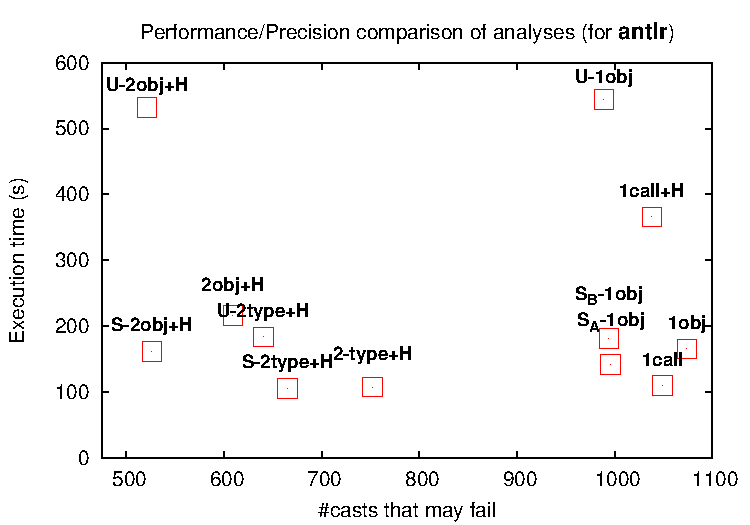
\includegraphics[width=\textwidth]{assets/hybrid/antlr.pdf}
\end{subfigure}\hspace{1cm}%
\begin{subfigure}[b]{0.45\textwidth}
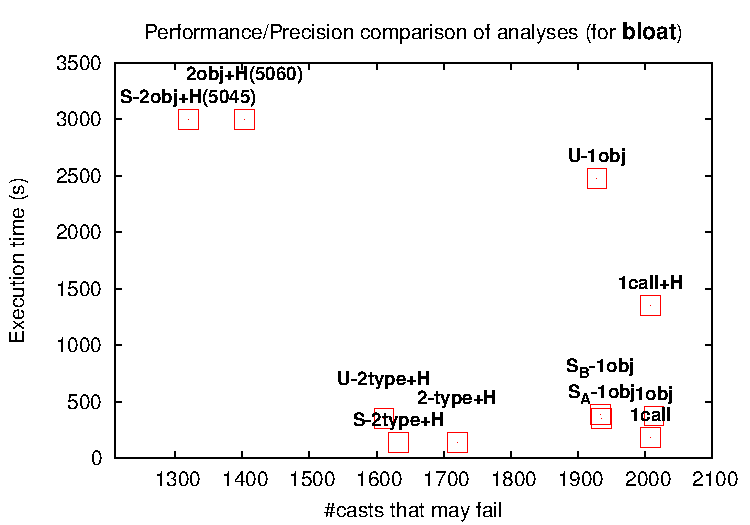
\includegraphics[width=\textwidth]{assets/hybrid/bloat.pdf}
\end{subfigure}

\begin{subfigure}[b]{0.45\textwidth}
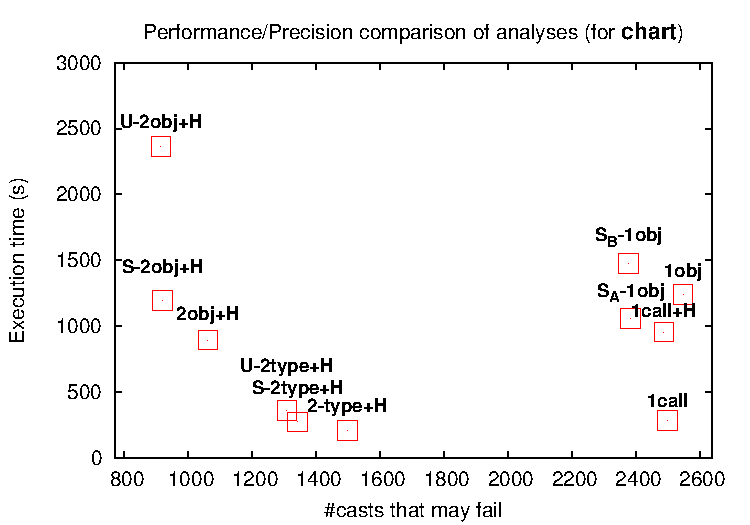
\includegraphics[width=\textwidth]{assets/hybrid/chart.pdf}
\end{subfigure}\hspace{1cm}%
\begin{subfigure}[b]{0.45\textwidth}
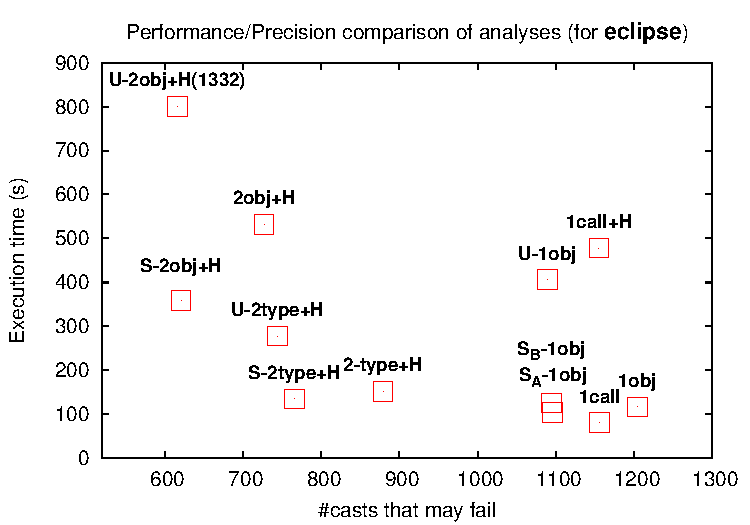
\includegraphics[width=\textwidth]{assets/hybrid/eclipse.pdf}
\end{subfigure}

\begin{subfigure}[b]{0.45\textwidth}
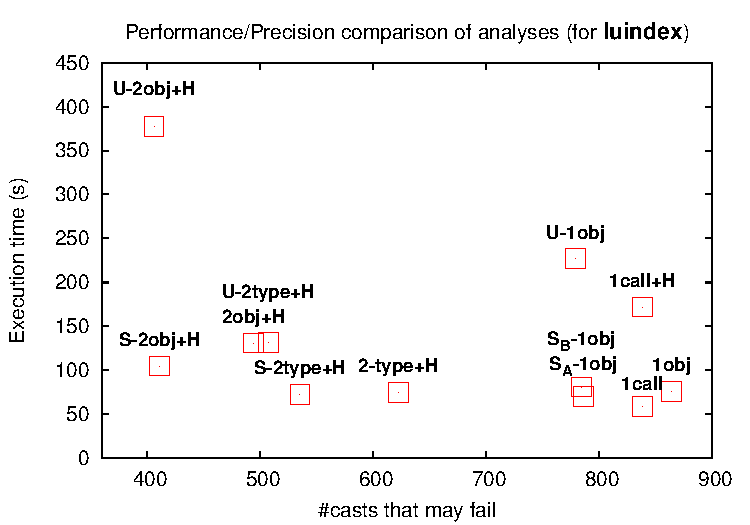
\includegraphics[width=\textwidth]{assets/hybrid/luindex.pdf}
\end{subfigure}\hspace{1cm}%
\begin{subfigure}[b]{0.45\textwidth}
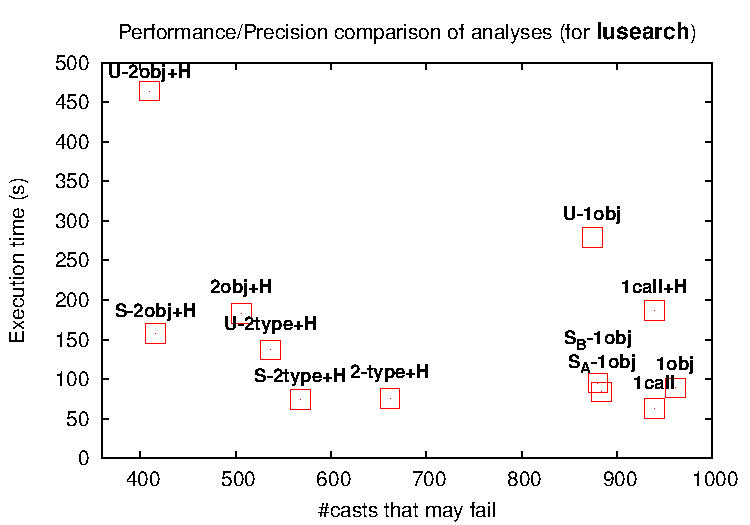
\includegraphics[width=\textwidth]{assets/hybrid/lusearch.pdf}
\end{subfigure}

\begin{subfigure}[b]{0.45\textwidth}
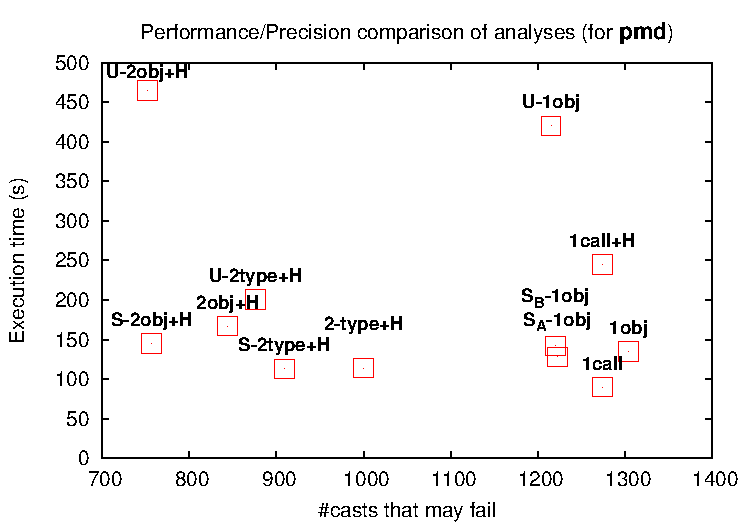
\includegraphics[width=\textwidth]{assets/hybrid/pmd.pdf}
\end{subfigure}\hspace{1cm}%
\begin{subfigure}[b]{0.45\textwidth}
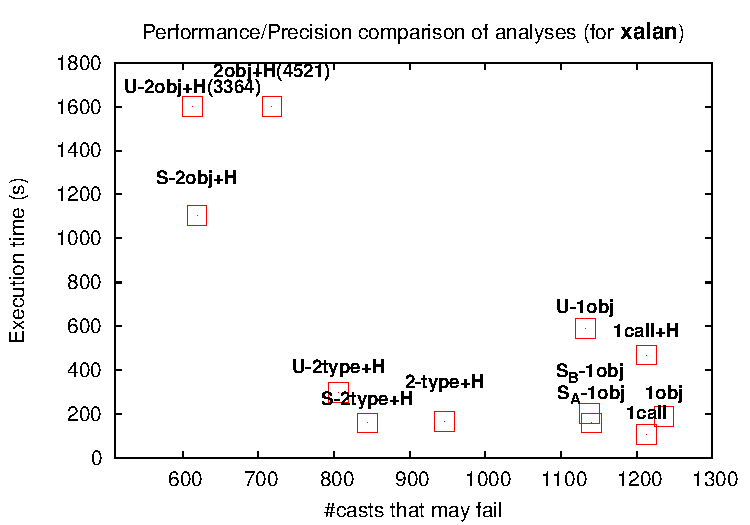
\includegraphics[width=\textwidth]{assets/hybrid/xalan.pdf}
\end{subfigure}
\caption{Graphical depiction of performance vs. precision metrics for eight of our benchmarks over all analyses. Lower is better on both axes. The Y axis is truncated for readability. Out-of-bounds points are included at lower Y values, with their real running time in parentheses.}
\label{fig:hybrid:precision}
\end{center}
\end{figure*}

For an illustration of the precision and performance spectrum, consider Figure~\ref{fig:hybrid:precision}, which plots analyses on precision/performance axes. The figure plots execution time against precision in the ``may-fail casts'' metric, i.e., the number of casts that the analysis cannot statically prove safe. Lower numbers are better on both axes, thus an analysis that is to the \textbf{left and below} another is better in both precision and performance. Values that are disproportionately high on the Y axis (i.e., large execution times) are clipped and plotted at the top of the figure, with the actual number included in parentheses. (Note that the Y axis starts at zero, while the X axis starts at an arbitrary point---we cannot know what is the ``ideal'' reference value for this metric.)

In terms of pre-existing analyses, Figure~\ref{fig:hybrid:precision} illustrates what has been past experience: 2obj+H is the most precise analysis, but often heavy. 1obj and 2type+H are both quite fast, with 2type+H also showing very good precision, often approaching 2obj+H. The two call-site-sensitive analyses (1call, 1call+H) are mostly shown for reference and to demonstrate the insights discussed in Section~\ref{sec:hybrid:main}. 1call is a fast analysis but vastly imprecise, while 1call+H is a bad tradeoff: its cost grows quite significantly relative to 1call without much precision added---call-site sensitivity is a bad choice for heap contexts.

As can be seen, the selective hybrid analyses (S$_A$-1obj, S$_A$-1obj, S-2obj+H, S-2type+H) usually offer an advantage over the corresponding base analysis (1obj, 2type+H, 2obj+H) in both precision and performance. In fact, selective hybrids are typically imperceptibly less precise than the corresponding uniform hybrid, yet much more precise than the base analysis. For instance, the plot points for S-2obj+H are always barely to the right of those for the theoretically more precise U-2obj+H (but significantly lower---uniform hybrids are very expensive), while they are clearly to the left of 2obj+H.


\subsection{Detailed Results}

Detailed results of our experiments are presented in Tables \ref{tab:hybrid:results-a} and \ref{tab:hybrid:results-b}. The tables show precision and performance metrics for all analyses. The precision metrics are:
\begin{inparaenum}[(1)]
\item the average points-to set size (i.e., average over all variables of their
points-to sets sizes),
\item the number of edges in the computed call-graph (which is typically a good proxy for the overall precision of the analysis, in broad strokes), and
the results of two client analyses:
\item the number of virtual calls that could not be de-virtualized, and
\item the number of casts that could not be statically proven safe.
\end{inparaenum}
A combination of these four metrics gives a reliable picture of the precision of an analysis. Note that the average points-to set size alone is not necessarily reliable, because it is influenced by a small number of library variables with enormous points-to sets. For comparison, the \emph{median} points-to set size is 1, for all analyses and benchmarks.

Performance is shown with two metrics:
\begin{inparaenum}[(1)]
\item time and
\item total size of all \emph{context-sensitive} points-to sets.
\end{inparaenum}
Although time is the ultimate performance metric, it is brittle: one can argue that our time measurements are influenced by a multitude of implementation or environment factors, among which are the choice of underlying data structures, indexing, and the overall implementation of the points-to analysis, especially since it is running on a Datalog engine, with its own complex implementation choices hidden. The context-sensitive points-to set size metric does not suffer from any such measurement or implementation bias. It is the foremost internal complexity metric of a points-to analysis, and typically correlates well with time, for analyses of the same flavor. Note that analysis implementations that fundamentally differ from ours also try hard to minimize this metric in order to achieve peak performance: Lhot\'{a}k's \textsc{Paddle} framework~\cite{thesis:Lhotak} is using binary decision diagrams (BDDs) for representing relations. The best BDD variable ordering (yielding ``impressive results'' \cite{pldi:2003:Berndl}) is one that minimizes the total size of context-sensitive points-to sets. In short, it is reasonable to expect that improvements in this internal metric reinforce the verdict of which analysis yields better performance, not just in our setting but generally. Furthermore, the size of context-sensitive points-to sets serves as a valuable indicator of the internally different computation performed by various analyses: Analyses with almost identical precision metrics (e.g., context-insensitive points-to set sizes, call-graph edges) have vastly different context-sensitive points-to set sizes.


\begin{table*}
\scalebox{0.8}{
\begin{tabular}{|r|c|l|p{1cm}|p{1cm}|p{1cm}!{\vrule width 2pt}l|l!{\vrule width 2pt}c|l|p{1cm}|p{1cm}|p{1cm}!{\vrule width 2pt}l|l|}

\cline{3-8}\cline{10-15}
\multicolumn{2}{c|}{} &
\rotatebox{90}{avg. objs per var} &
\rotatebox{90}{call-graph edges} &
\rotatebox{90}{polymorph v-calls} &
\rotatebox{90}{may-fail casts} &
\rotatebox{90}{elapsed time (s)} &
\rotatebox{90}{sensitive VPT (M)} &
\multicolumn{1}{c|}{} &
\rotatebox{90}{avg. objs per var} &
\rotatebox{90}{call-graph edges} &
\rotatebox{90}{polymorph v-calls} &
\rotatebox{90}{may-fail casts} &
\rotatebox{90}{elapsed time (s)} &
\rotatebox{90}{sensitive VPT (M)} \\

\cmidrule[2pt]{3-8}\cmidrule[2pt]{10-15}
\multicolumn{3}{c|}{} &
over 8.8K meths &
over 33K calls &
over 1.7K casts &
\multicolumn{4}{c|}{} &
over 10.2K meths &
over 31K calls &
over 2.8K casts &
\multicolumn{2}{c}{} \\
\cline{1-15}
1call & \multirow{13}{*}{\rotatebox{90}{\mbox{antlr}}} & 29.79 & 60999 & 1994 & 1049 & 110 & 16 & \multirow{13}{*}{\rotatebox{90}{\mbox{bloat}}} & 43.96 & 70506 & 2138 & 2008 & 186 & 32.9 \\
1call+H & & 29.58 & 60999 & 1994 & 1038 & 366 & 54.8 & & 43.94 & 70506 & 2138 & 2008 & 1351 & 150.5 \\
\cline{1-1}\cline{3-8}\cline{10-15}
1obj & & 24.86 & 60194 & 1933 & 1074 & 166 & 14.3 & & 41.26 & 69501 & 2076 & 2013 & 374 & 21.9 \\
U-1obj & & 24.55 & 60194 & 1933 & 989 & 544 & 65 & & 41.16 & 69501 & 2076 & 1928 & 2473 & 287.1 \\
S$_A$-1obj & & 24.90 & 60202 & 1936 & 996 & \best{142} & \best{10.5} & & 41.32 & 69511 & 2080 & 1935 & \best{353} & \best{20.1} \\
S$_B$-1obj & & 24.61 & 60194 & 1933 & 994 & 182 & 17.3 & & 41.18 & 69501 & 2076 & 1933 & 391 & 24 \\
\cline{1-1}\cline{3-8}\cline{10-15}
2obj+H & & 6.42 & 55548 & 1707 & 609 & 217 & 19.9 & & 13.25 & 60726 & 1640 & 1403 & 5060 & 153.5 \\
U-2obj+H & & 6.26 & 55548 & 1707 & 521 & 532 & 39.5 & & \bad{-} & \bad{-} & \bad{-} & \bad{-} & \bad{-} & \bad{-} \\
S-2obj+H & & 6.27 & 55548 & 1707 & 526 & \best{162} & \best{13.9} & & 13.10 & 60726 & 1640 & 1320 & \best{5045} & \best{149.8} \\
\cline{1-1}\cline{3-8}\cline{10-15}
2type+H & & 17.60 & 55850 & 1759 & 752 & 108 & 5.3 & & 16.28 & 62115 & 1888 & 1720 & 142 & 11.4 \\
U-2type+H & & 7.14 & 55765 & 1746 & 640 & 184 & 8.9 & & 14.71 & 61753 & 1827 & 1611 & 353 & 30.3 \\
S-2type+H & & 17.39 & 55850 & 1759 & 665 & \best{106} & \best{4.8} & & 16.10 & 62115 & 1888 & 1633 & \best{140} & \best{11} \\

\cmidrule[2pt]{1-15}
\multicolumn{3}{c|}{} &
over 15K meths &
over 35K calls &
over 3.5K casts &
\multicolumn{4}{c|}{} &
over 9.3K meths &
over 23K calls &
over 2K casts &
\multicolumn{2}{c}{} \\
\cline{1-15}
1call & \multirow{13}{*}{\rotatebox{90}{\mbox{chart}}} & 45.12 & 82156 & 2900 & 2500 & 288 & 49.6 & \multirow{13}{*}{\rotatebox{90}{\mbox{eclipse}}} & 21.84 & 53006 & 1515 & 1156 & 81 & 12.3 \\
1call+H & & 45.11 & 82078 & 2897 & 2488 & 957 & 120.9 & & 21.65 & 53001 & 1514 & 1155 & 478 & 61.5 \\
\cline{1-1}\cline{3-8}\cline{10-15}
1obj & & 40.80 & 81423 & 2821 & 2548 & 1240 & 62.5 & & 18.65 & 52114 & 1429 & 1204 & 117 & 9.4 \\
U-1obj & & \bad{-} & \bad{-} & \bad{-} & \bad{-} & \bad{-} & \bad{-} & & 18.41 & 51935 & 1404 & 1089 & 406 & 42.3 \\
S$_A$-1obj & & 40.72 & 81075 & 2815 & 2385 & \best{1059} & \best{39.7} & & 18.59 & 51958 & 1412 & 1096 & \best{105} & \best{7.6} \\
S$_B$-1obj & & 40.11 & 81012 & 2808 & 2378 & 1477 & 89.7 & & 18.43 & 51936 & 1404 & 1094 & 126 & 10.8 \\
\cline{1-1}\cline{3-8}\cline{10-15}
2obj+H & & 5.30 & 59162 & 1610 & 1062 & \best{896} & 67.6 & & 5.75 & 44900 & 1163 & 727 & 532 & 44.6 \\
U-2obj+H & & 4.99 & 59142 & 1603 & 915 & 2363 & 115.7 & & 5.60 & 44899 & 1163 & 616 & 1332 & 89.8 \\
S-2obj+H & & 5.00 & 59152 & 1610 & 920 & 1199 & \best{53} & & 5.61 & 44900 & 1163 & 621 & \best{359} & \best{32.3} \\
\cline{1-1}\cline{3-8}\cline{10-15}
2type+H & & 7.02 & 62290 & 1775 & 1498 & \best{211} & \best{13.3} & & 7.93 & 45318 & 1233 & 879 & 152 & 13.6 \\
U-2type+H & & 5.89 & 62172 & 1756 & 1309 & 362 & 21.3 & & 6.41 & 45123 & 1202 & 744 & 278 & 24.4 \\
S-2type+H & & 6.57 & 62280 & 1775 & 1343 & 276 & 16.5 & & 7.61 & 45235 & 1229 & 766 & \best{135} & \best{11.5} \\

\cmidrule[2pt]{1-15}
\multicolumn{3}{c|}{} &
over 10K meths &
over 26K calls &
over 2K casts &
\multicolumn{4}{c|}{} &
over 8.5K meths &
over 21K calls &
over 1.9K casts &
\multicolumn{2}{c}{} \\
\cline{1-15}
1call & \multirow{13}{*}{\rotatebox{90}{\mbox{hsqldb}}} & 18.56 & 54619 & 1552 & 1360 & 90 & 9.6 & \multirow{13}{*}{\rotatebox{90}{\mbox{jython}}} & 20.64 & 50494 & 1525 & 1140 & 88 & 10.4 \\
1call+H & & 18.53 & 54619 & 1552 & 1360 & 332 & 39.8 & & 20.57 & 50480 & 1524 & 1140 & 401 & 50.6 \\
\cline{1-1}\cline{3-8}\cline{10-15}
1obj & & 15.41 & 53726 & 1480 & 1385 & 218 & 13.9 & & 18.21 & 49622 & 1448 & 1157 & 119 & 8.7 \\
U-1obj & & 15.30 & 53724 & 1479 & 1302 & 1351 & 74.3 & & 18.01 & 49614 & 1448 & 1087 & 375 & 43.2 \\
S$_A$-1obj & & 15.58 & 53730 & 1482 & 1320 & \best{183} & \best{9.6} & & 18.19 & 49622 & 1453 & 1094 & 138 & \best{6.7} \\
S$_B$-1obj & & 15.32 & 53724 & 1479 & 1308 & 329 & 29.5 & & 18.09 & 49614 & 1448 & 1092 & 138 & 10.8 \\
\cline{1-1}\cline{3-8}\cline{10-15}
2obj+H & & \bad{-} & \bad{-} & \bad{-} & \bad{-} & \bad{-} & \bad{-} & & \bad{-} & \bad{-} & \bad{-} & \bad{-} & \bad{-} & \bad{-} \\
U-2obj+H & & \bad{-} & \bad{-} & \bad{-} & \bad{-} & \bad{-} & \bad{-} & & \bad{-} & \bad{-} & \bad{-} & \bad{-} & \bad{-} & \bad{-} \\
S-2obj+H & & \bad{-} & \bad{-} & \bad{-} & \bad{-} & \bad{-} & \bad{-} & & \bad{-} & \bad{-} & \bad{-} & \bad{-} & \bad{-} & \bad{-} \\
\cline{1-1}\cline{3-8}\cline{10-15}
2type+H & & 7.92 & 49421 & 1276 & 1031 & \best{195} & \best{13.7} & & 8.55 & 43269 & 1268 & 909 & 731 & \best{52} \\
U-2type+H & & 6.71 & 49319 & 1263 & 923 & 583 & 42.9 & & 7.18 & 43138 & 1236 & 822 & 1363 & 118.4 \\
S-2type+H & & 7.74 & 49421 & 1276 & 948 & 238 & 20.5 & & 8.30 & 43269 & 1268 & 840 & \best{676} & 56.5 \\
\cline{1-15}

\end{tabular}
} % end scalebox
\caption[]{Precision and performance metrics for all benchmarks and analyses, grouped by relevance. Continues in Table~\ref{tab:hybrid:results-b}.}
\label{tab:hybrid:results-a}
\end{table*}

\begin{table*}
\scalebox{0.8}{
\begin{tabular}{|r|c|l|p{1cm}|p{1cm}|p{1cm}!{\vrule width 2pt}l|l!{\vrule width 2pt}c|l|p{1cm}|p{1cm}|p{1cm}!{\vrule width 2pt}l|l|}

\cline{3-8}\cline{10-15}
\multicolumn{2}{c|}{} &
\rotatebox{90}{avg. objs per var} &
\rotatebox{90}{call-graph edges} &
\rotatebox{90}{polymorph v-calls} &
\rotatebox{90}{may-fail casts} &
\rotatebox{90}{elapsed time (s)} &
\rotatebox{90}{sensitive VPT (M)} &
\multicolumn{1}{c|}{} &
\rotatebox{90}{avg. objs per var} &
\rotatebox{90}{call-graph edges} &
\rotatebox{90}{polymorph v-calls} &
\rotatebox{90}{may-fail casts} &
\rotatebox{90}{elapsed time (s)} &
\rotatebox{90}{sensitive VPT (M)} \\

\cmidrule[2pt]{3-8}\cmidrule[2pt]{10-15}
\multicolumn{3}{c|}{} &
over 7.9K meths &
over 18K calls &
over 1.4K casts &
\multicolumn{4}{c|}{} &
over 8.4K meths &
over 19K calls &
over 1.5K casts &
\multicolumn{2}{c}{} \\
\cline{1-15}
1call & \multirow{13}{*}{\rotatebox{90}{\mbox{luindex}}} & 17.65 & 41992 & 1180 & 838 & 59 & 7.8 & \multirow{13}{*}{\rotatebox{90}{\mbox{lusearch}}} & 18.64 & 45270 & 1360 & 939 & 63 & 8.7 \\
1call+H & & 17.58 & 41992 & 1180 & 838 & 172 & 26.1 & & 18.47 & 45270 & 1360 & 939 & 187 & 28.5 \\
\cline{1-1}\cline{3-8}\cline{10-15}
1obj & & 14.94 & 41103 & 1119 & 864 & 76 & 5.4 & & 15.71 & 44371 & 1299 & 961 & 89 & 6.2 \\
U-1obj & & 14.81 & 41103 & 1119 & 779 & 227 & 26.3 & & 15.57 & 44365 & 1299 & 874 & 279 & 30.3 \\
S$_A$-1obj & & 14.97 & 41111 & 1122 & 786 & \best{70} & \best{4.1} & & 15.79 & 44379 & 1302 & 884 & \best{84} & \best{5.3} \\
S$_B$-1obj & & 14.83 & 41103 & 1119 & 784 & 81 & 6.4 & & 15.60 & 44371 & 1299 & 880 & 95 & 7.2 \\
\cline{1-1}\cline{3-8}\cline{10-15}
2obj+H & & 4.77 & 36580 & 894 & 494 & 131 & 11.1 & & 4.71 & 39452 & 1065 & 506 & 183 & 13.2 \\
U-2obj+H & & 4.55 & 36580 & 894 & 406 & 377 & 22.4 & & 4.49 & 39446 & 1065 & 410 & 464 & 26.3 \\
S-2obj+H & & 4.55 & 36580 & 894 & 411 & \best{105} & \best{7.2} & & 4.50 & 39452 & 1065 & 416 & \best{158} & \best{10} \\
\cline{1-1}\cline{3-8}\cline{10-15}
2type+H & & 6.20 & 36889 & 949 & 622 & 75 & 4.5 & & 6.13 & 39763 & 1122 & 662 & 76 & 4.2 \\
U-2type+H & & 5.15 & 36796 & 932 & 507 & 132 & 7.6 & & 5.10 & 39662 & 1103 & 537 & 137 & 7.8 \\
S-2type+H & & 5.92 & 36889 & 949 & 535 & \best{73} & \best{3.5} & & 5.86 & 39763 & 1122 & 568 & \best{74} & \best{3.6} \\

\cmidrule[2pt]{1-15}
\multicolumn{3}{c|}{} &
over 9.2K methss &
over 21K calls &
over 2K casts &
\multicolumn{4}{c|}{} &
over 10.5K meths &
over 26K calls &
over 2K casts &
\multicolumn{2}{c}{} \\
\cline{1-15}
1call & \multirow{13}{*}{\rotatebox{90}{\mbox{pmd}}} & 19.94 & 49097 & 1249 & 1274 & 90 & 11.4 & \multirow{13}{*}{\rotatebox{90}{\mbox{xalan}}} & 25.50 & 57168 & 1976 & 1213 & 108 & 14.5 \\
1call+H & & 19.82 & 49097 & 1249 & 1274 & 245 & 35.9 & & 25.38 & 57168 & 1976 & 1213 & 470 & 59.8 \\
\cline{1-1}\cline{3-8}\cline{10-15}
1obj & & 17.36 & 48250 & 1187 & 1304 & 135 & 7.9 & & 21.86 & 56412 & 1920 & 1236 & 189 & 15.5 \\
U1obj & & 17.22 & 48250 & 1187 & 1215 & 420 & 42.6 & & 21.59 & 56158 & 1905 & 1132 & 591 & 67.5 \\
S$_A$1obj & & 17.37 & 48258 & 1190 & 1222 & \best{128} & \best{6.9} & & 21.84 & 56404 & 1921 & 1140 & \best{161} & \best{10.9} \\
S$_B$1obj & & 17.24 & 48250 & 1187 & 1220 & 142 & 9.2 & & 21.69 & 56395 & 1918 & 1138 & 205 & 18.2 \\
\cline{1-1}\cline{3-8}\cline{10-15}
2obj+H & & 4.87 & 43068 & 937 & 844 & 167 & 13.2 & & 5.48 & 50148 & 1619 & 718 & 4521 & 166.6 \\
U2obj+H & & 4.68 & 43067 & 937 & 752 & 465 & 30.5 & & 5.22 & 50054 & 1615 & 613 & 3364 & 171.7 \\
S2obj+H & & 4.68 & 43067 & 937 & 757 & \best{145} & \best{10} & & 5.23 & 50054 & 1615 & 619 & \best{1105} & \best{63.3} \\
\cline{1-1}\cline{3-8}\cline{10-15}
2type+H & & 6.35 & 43401 & 988 & 1000 & 114 & 4.5 & & 7.52 & 50539 & 1677 & 946 & 168 & 10.2 \\
U2type+H & & 5.28 & 43315 & 976 & 876 & 201 & 9.7 & & 6.19 & 50432 & 1660 & 806 & 299 & 17.4 \\
S2type+H & & 6.10 & 43400 & 988 & 909 & \best{113} & \best{3.9} & & 7.16 & 50526 & 1677 & 844 & \best{161} & \best{9} \\
\cline{1-15}
\end{tabular}
} % end scalebox
\caption[]{Precision and performance metrics for all benchmarks and analyses, grouped by relevance. In all cases \textbf{lower is better}. Dash (-) entries are for analyses that did not terminate in 90mins. The 4 precision metrics shown are the average size of points-to sets (how many heap objects are computed to be pointed-to per-var), the number of edges in the computed call-graph, the number of virtual calls whose target cannot be disambiguated by the analysis, and the number of casts that cannot be statically shown safe by the analysis. Reference numbers (e.g., total reachable casts in the program) are shown in parentheses in the metric's heading. These numbers change little per-analysis. Performance is shown as running time and size of context-sensitive var-points-to data (the main platform-independent internal complexity metric). Best performance numbers per-analysis-group are \best{in bold}.}
\label{tab:hybrid:results-b}
\end{table*}

Since Tables~\ref{tab:hybrid:results-a}-\ref{tab:hybrid:results-b} have a high information density, we guide the reader through some of the most important findings below (see also a partial illustration in Figure~\ref{fig:hybrid:precision}).

\begin{itemize}
\item \textbf{\emph{General observations.}}
The analyses shown are in 4 groups of closely related analyses: call-site sensitive, 1-object-sensitive, 2-object-sensitive with a 1-context-sensitive heap, and 2-type-sensitive with a 1-context-sensitive heap. These analyses span a large performance and precision spectrum. For instance, for the chart benchmark, the least precise analysis, 1call, runs for under 5mins and computes an average points-to size of over 45, while the most precise, U-2obj+H, runs for over 53mins and computes an average points-to size of under 5. The difference in precision is also vividly shown in the ``may-fail casts'' metric: the 1call analysis cannot prove 2500 casts safe, while the U-2obj+H fails to prove safe just 915 casts (both numbers from a total of about 3.5K reachable casts---the exact number varies slightly due to method reachability variation per analysis). 

Specifically, 1call, 1obj, and 2type+H are the fastest analyses in our set (for different programs each), with each one offering significant precision enhancements relative to the previous. 2obj+H is typically slower but manageable, and achieves very high precision.

\item \textbf{\emph{Uniform hybrid analyses.}}
Recall that uniform hybrid analyses (U-1obj, U-2obj+H, U-2type+H) were defined to always keep a combination of object-sensitive and call-site-sensitive context. As a result, the analyses are more precise than their respective base analyses (1obj, 2obj+H, 2type+H), especially in the ``may-fail casts'' metric. However, this precision comes at great cost: uniform hybrid analyses are often 3x or more slower than their base analyses with twice as large, or more, context-sensitive points-to sets. U-1obj and U-2obj+H are plainly bad tradeoffs in the design space: for a slight increase in precision, the performance cost is heavy.

U-2type+H is a bit more reasonable: it achieves more significant precision gains and its performance toll is often under 2x while still terminating comfortably for all our benchmarks. In fact, a surprising finding was that U-2type+H is a tempting alternative to 2obj+H for applications that need very high precision, given its good scalability. A possible explanation is due to the specific nature of type-sensitive analyses: the class in which a receiver object is allocated forms a good differentiator of behavior when combined with a call-site.

\item \textbf{\emph{1obj hybrids.}}
We presented two selective hybrids of a 1-object-sensitive analysis: S$_A$-1obj (which keeps either an allocation site or a call-site as context, but not both) and S$_B$-1obj (which always keeps an allocation site as context and occasionally adds a call-site to it). They both turn out to be interesting analyses from a practical standpoint. The former is consistently faster than the base 1obj analysis, with roughly similar precision and occasionally (for the ``may-fail casts'' metric) higher precision. The size of context-sensitive points-to sets also confirms that this is a ``lighter'' analysis that is likely to cost less in any context. The S$_B$-1obj analysis is always more precise than 1obj (as is statically guaranteed) for a slight extra cost. Indeed, S$_B$-1obj is a good approximation of the uniform hybrid analysis, U-1obj, in terms of precision, for a fraction (typically less than a third) of the cost.

\item \textbf{\emph{2obj+H hybrids.}}
The selective hybrid idea yields even more dividends when applied to the very precise 2obj+H analysis. S-2obj+H is more precise than 2obj+H and only very slightly less precise than the uniform hybrid, U-2obj+H. In terms of performance, however, the analysis is typically well over 3 times faster than U-2obj+H, and significantly faster (an average of 53\% speedup) than 2obj+H. This is interesting, given the practical value of 2obj+H, since it establishes a new sweet spot in the space of relatively scalable but highly precise analyses: S-2obj+H is both more precise than 2obj+H (especially for ``may-fail casts'') and substantially faster.

\item \textbf{\emph{2type+H hybrids.}}
The 2type+H analysis variations are also highly interesting in practice. This is an analysis space that yields excellent precision relative to its low cost. There are few cases in which one might prefer some other inexpensive analysis over 2type+H given the combination of precision and competitive performance of the latter. As we saw, the uniform hybrid, U-2type+H, is an interesting tradeoff in this space. The selective hybrid, S-2type+H, also performs quite well. It is just as fast or slightly faster than the base analysis 2type+H, while also being more precise.
\end{itemize}


\section{Conclusions and Future Work}

This chapter presented a comprehensive map for the exploration of context combinations in points-to analysis, and used it to discover several interesting design points. Object-sensitivity and call-site-sensitivity had never been fruitfully combined in the past, although the idea is clearly tempting. We speculate that the reasons for the paucity of hybrid context-sensitivity results have been a) the difficulty of having a good enough model for the space of combinations and a convenient implementation to explore it; b) a belief that nothing fruitful will come out of such a combination, because call-site sensitivity incurs a high performance cost, which is more profitably spent on an extra level of object-sensitivity. The latter insight is mostly true, but only if one considers uniform hybrid analyses. As we saw, much of the benefit of call-site and object-sensitive hybrids comes from allowing the context to vary between pure object-sensitive and extended. The result of our work has been new sweet spots, in both precision and performance, for some of the most practically relevant analysis variations.

There are several interesting directions for further work that open up. First, our model gives the ability for further experimentation, e.g., with deeper-context analyses. Furthermore, it is interesting to examine if a hybrid context should perhaps change form more aggressively. The \consname{Merge} and \consname{MergeStatic} functions could examine the context passed to them as argument and create different kinds of contexts in return. For instance, the context of a statically called method could have a different form (e.g., more elements) for a call made inside another statically called method vs. a call made in a virtual method. Similarly, objects could have different context, via the \consname{Record} function, depending on the context form of their allocating method. To explore this space without blind guessing, one needs to understand what programming patterns are best handled by hybrid contexts and how. For deep contexts this remains a challenge, as it is hard to reason about how context elements affect precision. (E.g., past work had to offer involved arguments for why the allocator object of the receiver object of a method is a better context element than the caller object  \cite{popl:2011:Smaragdakis}.) This challenge is, however, worth addressing for the next level of benefit in context-sensitive points-to analysis.